\begin{figure}
\centering
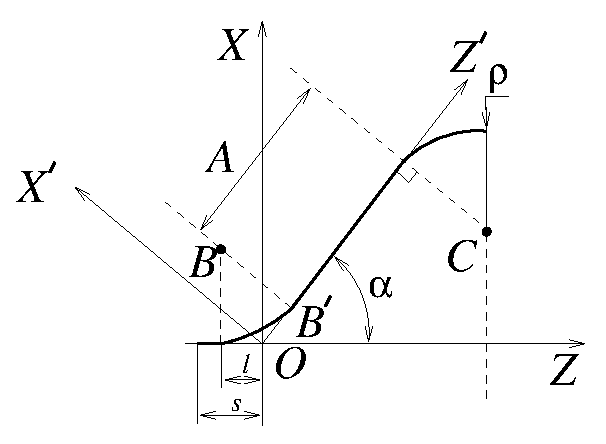
\includegraphics{bqwave_prime.eps}
\caption{Calculation of the distance $d$ from point $(z, x)$ to the
fan's neutral fibre, in the case of the starting quarter-wave.
If $z < -l\/$ and the input point is below the $BB^{\prime}\/$ line, then $d = x$.
If $z^{\prime} < l\/$, then $d =
\sqrt{(x^{\prime}-\rho)^2 + (z^{\prime}-l)^2} - 
\rho\/$, if $z^{\prime}< A\/$, then  $d=x^{\prime}\/$,
else $d = \sqrt{(x^{\prime} + \rho)^2 +
(z^{\prime}-(A + l))^2} - \rho\/$. } 
\label{bqwave_prime}
\end{figure}
